% ============================================================
% 第7章：三角函数（下）——正切、恒等式、反三角
% ============================================================

\chapter{三角函数（下）——正切、恒等式、反三角}

\begin{applicationbox}
\textbf{学完本章你能做什么？}
\begin{enumerate}
  \item 学会 \(\tan x\) 的图像和性质，能对比 \(\sin, \cos, \tan\) 的异同
  \item 掌握三角恒等式——和差角公式、倍角公式——它们是 AI 中 RoPE 位置编码的基础
  \item 会使用反三角函数 \(\arcsin, \arccos, \arctan\)——从三角函数值反推角度
\end{enumerate}
\end{applicationbox}


% ============================================================
\section{从第6章来——还需要更多}
% ============================================================

第6章我们学了 \(\sin x\) 和 \(\cos x\)——最基本的两个三角函数。

但还有 \(\tan x\)、更多的恒等式、以及逆运算（反三角函数）需要掌握。\\
这些知识在 Transformer 的位置编码（RoPE）、傅里叶变换、信号处理中都会用到。


% ============================================================
\section{正切函数 \(\tan x\)}
% ============================================================

\begin{definitionbox}[正切函数]
\[
\tan x = \frac{\sin x}{\cos x}, \quad \cos x \neq 0
\]

读作"tan x"（摊进塔 x），英文 tangent。
\end{definitionbox}

\begin{examplebox}[1——\(\tan x\) 的图像]
\begin{center}
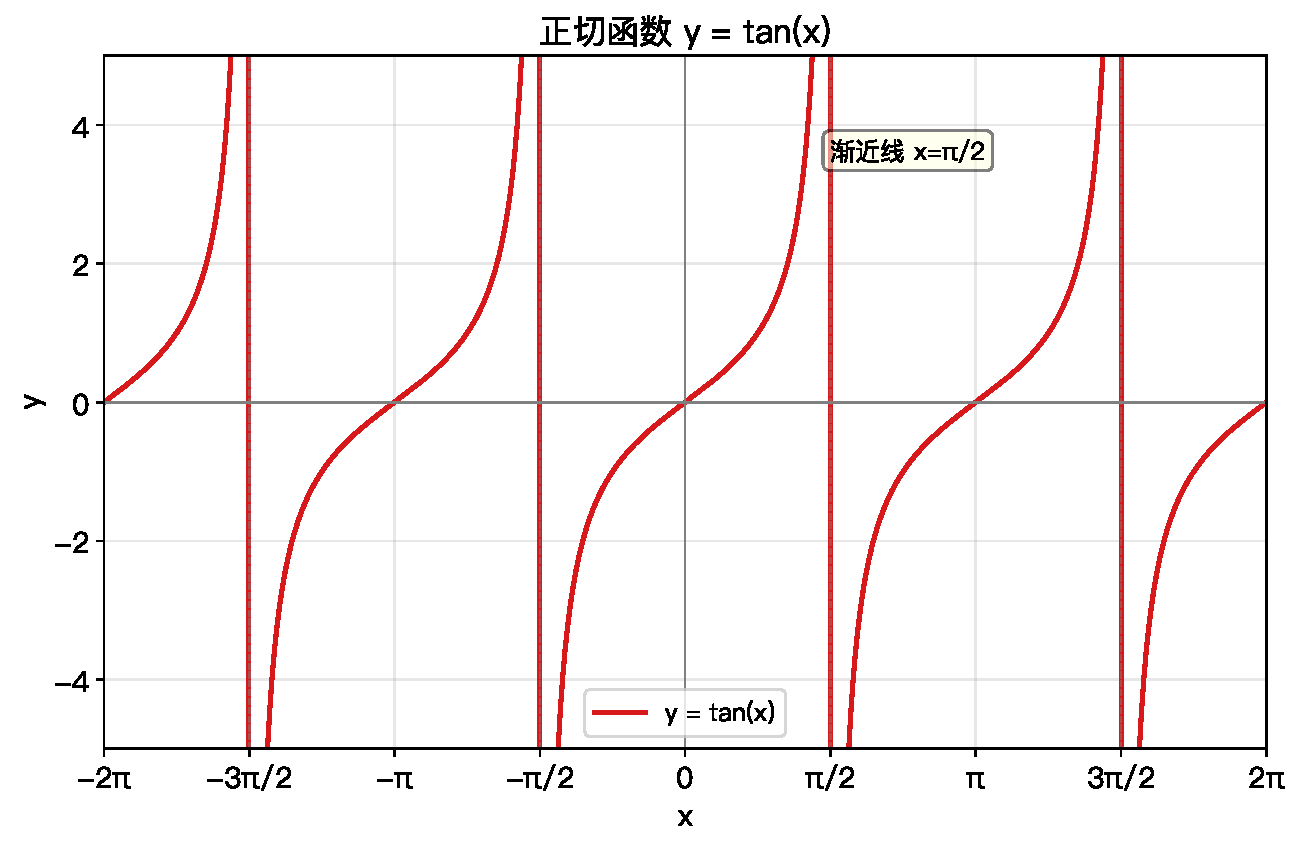
\includegraphics[width=0.85\textwidth]{figures/ch07_tangent.pdf}
\end{center}

\textbf{关键特征：}
\begin{enumerate}
  \item \textbf{周期}：\(\pi\)（不是 \(2\pi\)！）——因为 \(\tan(x+\pi) = \tan x\)
  \item \textbf{定义域}：\(x \neq \dfrac{\pi}{2} + n\pi\)（\(\cos x = 0\) 的点）
  \item \textbf{值域}：\(\mathbb{R}\)（可以取任意实数）
  \item \textbf{渐近线}：在 \(x = \dfrac{\pi}{2} + n\pi\) 处有垂直渐近线
  \item \textbf{奇函数}：\(\tan(-x) = -\tan x\)
  \item \textbf{特殊值}：\(\tan 0 = 0\)，\(\tan \dfrac{\pi}{4} = 1\)，\(\tan \pi = 0\)
\end{enumerate}
\end{examplebox}


% ============================================================
\section{\(\sin, \cos, \tan\) 对比}
% ============================================================

\begin{examplebox}[2——三大三角函数同框]
\begin{center}
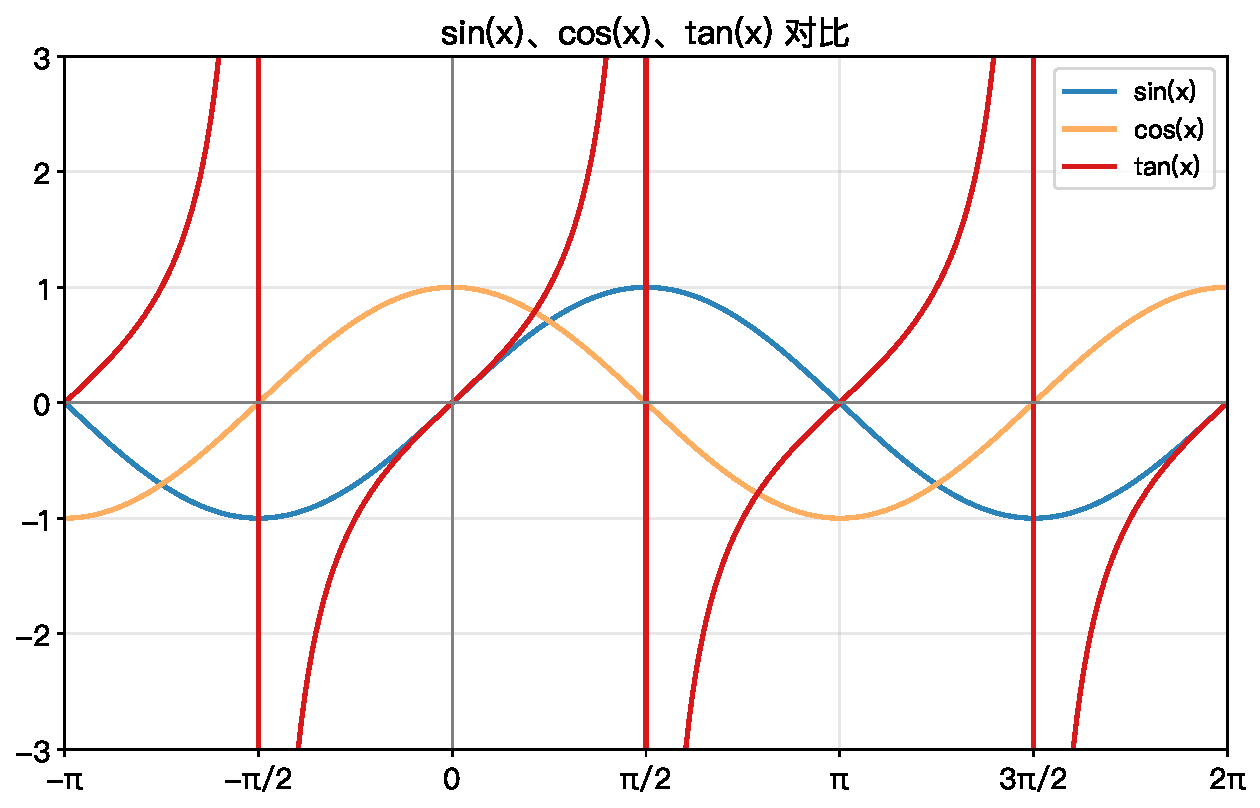
\includegraphics[width=0.85\textwidth]{figures/ch07_sin_cos_tan.pdf}
\end{center}

\begin{center}
\begin{tabular}{c|c|c|c}
 & \(\sin x\) & \(\cos x\) & \(\tan x\) \\
\hline
定义域 & \(\mathbb{R}\) & \(\mathbb{R}\) & \(x \neq \pi/2 + n\pi\) \\
值域 & \([-1, 1]\) & \([-1, 1]\) & \(\mathbb{R}\) \\
周期 & \(2\pi\) & \(2\pi\) & \(\pi\) \\
奇偶性 & 奇 & 偶 & 奇 \\
零点 & \(n\pi\) & \(\pi/2 + n\pi\) & \(n\pi\) \\
\end{tabular}
\end{center}
\end{examplebox}


% ============================================================
\section{三角恒等式——最重要的公式}
% ============================================================

\subsection{和差角公式}

\begin{theorembox}[和差角公式]
\begin{align*}
\sin(a \pm b) &= \sin a \cos b \pm \cos a \sin b \\
\cos(a \pm b) &= \cos a \cos b \mp \sin a \sin b \\
\tan(a \pm b) &= \frac{\tan a \pm \tan b}{1 \mp \tan a \tan b}
\end{align*}
\end{theorembox}

\begin{examplebox}[3——用和差角公式求 \(\sin 75^\circ\)]
\[
\sin 75^\circ = \sin(45^\circ + 30^\circ) = \sin 45^\circ \cos 30^\circ + \cos 45^\circ \sin 30^\circ
\]
\[
= \frac{\sqrt{2}}{2} \cdot \frac{\sqrt{3}}{2} + \frac{\sqrt{2}}{2} \cdot \frac{1}{2}
= \frac{\sqrt{6} + \sqrt{2}}{4} \approx 0.9659
\]

\textbf{验证：} 计算器 \(\sin 75^\circ \approx 0.9659\) [OK]
\end{examplebox}

\subsection{倍角公式}

\begin{theorembox}[倍角公式]
由和差角公式令 \(a = b = x\) 得到：
\begin{align*}
\sin 2x &= 2\sin x \cos x \\
\cos 2x &= \cos^2 x - \sin^2 x = 1 - 2\sin^2 x = 2\cos^2 x - 1
\end{align*}
\end{theorembox}

\begin{examplebox}[4——倍角公式的应用]
已知 \(\sin x = \dfrac{3}{5}\)（\(x\) 在第一象限），求 \(\sin 2x\)。

解：
\[
\cos x = \sqrt{1 - \sin^2 x} = \sqrt{1 - \frac{9}{25}} = \sqrt{\frac{16}{25}} = \frac{4}{5}
\]
\[
\sin 2x = 2\sin x \cos x = 2 \cdot \frac{3}{5} \cdot \frac{4}{5} = \frac{24}{25}
\]
\end{examplebox}

\subsection{半角公式}

\begin{theorembox}[半角公式]
由倍角公式变形得到：
\[
\sin^2 \frac{x}{2} = \frac{1 - \cos x}{2}, \qquad
\cos^2 \frac{x}{2} = \frac{1 + \cos x}{2}
\]
\end{theorembox}


% ============================================================
\section{反三角函数——从值反推角度}
% ============================================================

如果 \(\sin \theta = 0.5\)，那 \(\theta\) 是多少？\\
我们知道 \(\theta = \pi/6\) 是一个答案，但还有 \(\theta = 5\pi/6\)……有无穷多个。

我们需要\textbf{限制值域}，使反函数成为单值函数。

\begin{definitionbox}[反三角函数]
\begin{center}
\begin{tabular}{c|c|c}
\textbf{函数} & \textbf{定义域} & \textbf{值域} \\
\hline
\(y = \arcsin x\)（或 \(\sin^{-1} x\)） & \([-1, 1]\) & \([-\pi/2,\; \pi/2]\) \\
\(y = \arccos x\)（或 \(\cos^{-1} x\)） & \([-1, 1]\) & \([0,\; \pi]\) \\
\(y = \arctan x\)（或 \(\tan^{-1} x\)） & \(\mathbb{R}\) & \((-\pi/2,\; \pi/2)\) \\
\end{tabular}
\end{center}

\textbf{读法：} \(\arcsin x\) 读作"阿克赛因 x"，\(\arccos x\) 读作"阿克扣赛因 x"。
\end{definitionbox}

\begin{examplebox}[5——\(\arcsin x\) 和 \(\arccos x\)]
\begin{center}
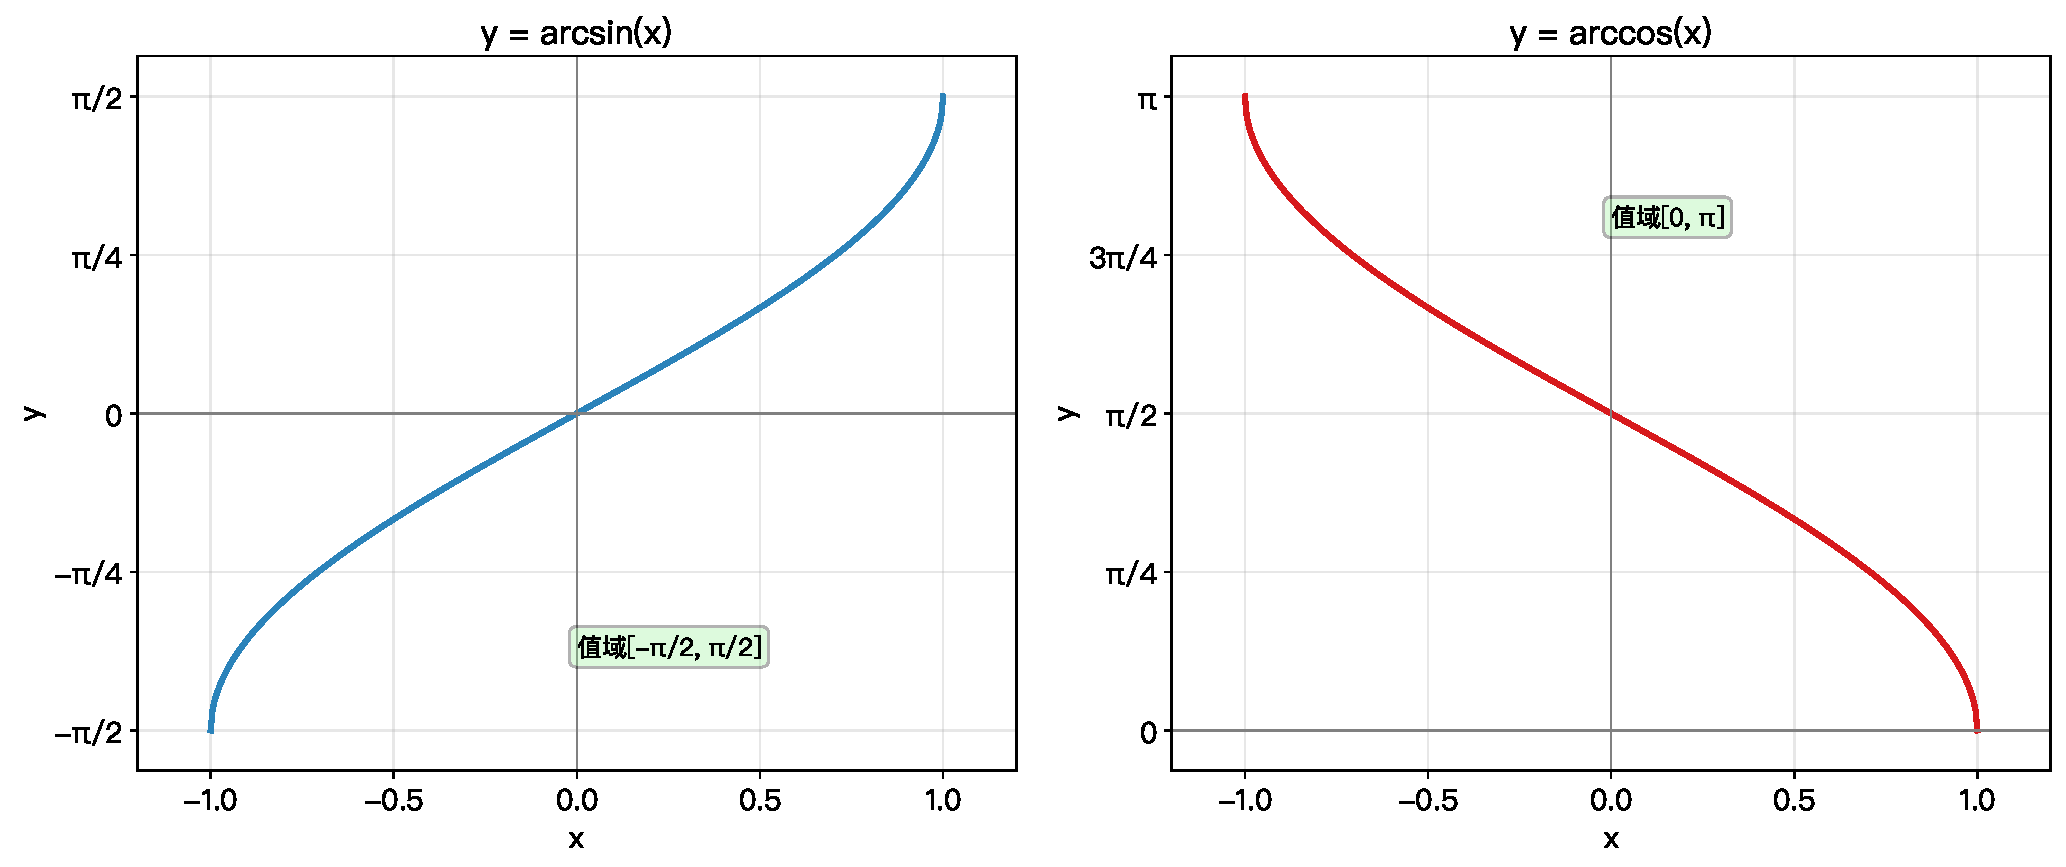
\includegraphics[width=0.85\textwidth]{figures/ch07_arcsin_arccos.pdf}
\end{center}

\textbf{关键理解：}
\begin{itemize}
  \item \(\arcsin(0.5) = \dfrac{\pi}{6}\)（值域在 \([-\pi/2, \pi/2]\)，所以取 \(\pi/6\) 而不是 \(5\pi/6\)）
  \item \(\arccos(0.5) = \dfrac{\pi}{3}\)（值域在 \([0, \pi]\)）
  \item \(\arcsin(\sin x) = x\) 只在 \(x \in [-\pi/2, \pi/2]\) 时成立
\end{itemize}
\end{examplebox}

\begin{examplebox}[6——\(\arctan x\)]
\begin{center}
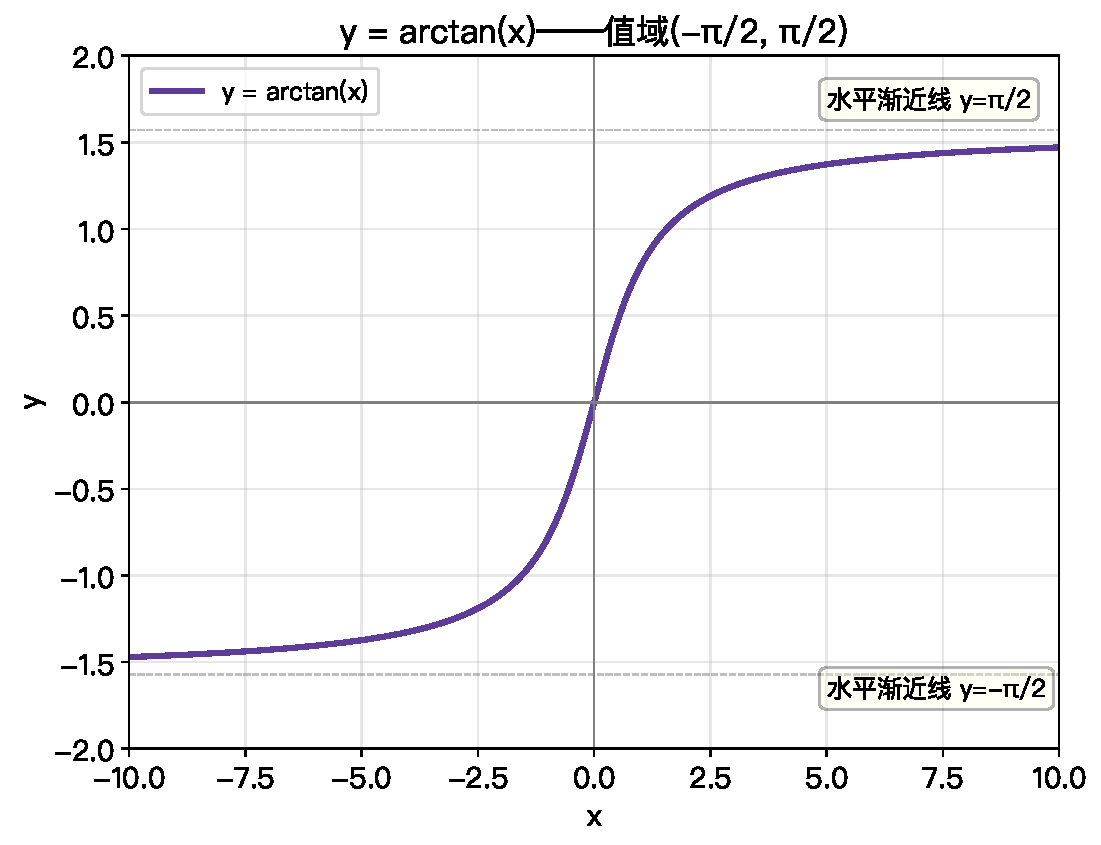
\includegraphics[width=0.55\textwidth]{figures/ch07_arctan.pdf}
\end{center}

\(\arctan x\) 的特点：
\begin{itemize}
  \item 定义域为全体实数，值域为 \((-\pi/2, \pi/2)\)
  \item 有两条水平渐近线：\(y = \pi/2\) 和 \(y = -\pi/2\)
  \item \(\arctan 1 = \pi/4\)，\(\arctan 0 = 0\)
  \item AI 中常用于将任意实数映射到有限范围（如 Sigmoid 的替代）
\end{itemize}
\end{examplebox}


% ============================================================
\section{三角函数在 AI 中的应用——RoPE 直觉}
% ============================================================

\begin{examplebox}[7——旋转位置编码 (RoPE)]
Transformer 模型需要知道词的位置信息。RoPE（旋转位置编码）用三角函数来编码位置：

\[
\text{位置 } m \text{ 的编码} = \begin{pmatrix}
\cos m\theta & -\sin m\theta \\
\sin m\theta & \cos m\theta
\end{pmatrix}
\begin{pmatrix}
x \\
y
\end{pmatrix}
\]

这其实就是\textbf{旋转}一个二维向量 \((x, y)\)——旋转的角度和位置 \(m\) 成正比。

\textbf{为什么用三角函数？}
\begin{enumerate}
  \item 旋转不改变向量长度（\(\sin^2 + \cos^2 = 1\)）
  \item 相对位置的关系可以用和差角公式简洁表达
  \item 位置越远，旋转角度越大
\end{enumerate}

这就是为什么 Transformer 能"知道"词与词的相对距离——三角函数在背后起了关键作用。
\end{examplebox}


% ============================================================
\section{符号卡片}
% ============================================================

\begin{symbolcard}
\(\tan x\) & \verb|\tan x| & 读作"tan x" & \(\sin x / \cos x\) \\
\(\arcsin x\) & \verb|\arcsin x| & 读作"阿克赛因" & \(\sin\) 的反函数，值域 \([-\pi/2,\pi/2]\) \\
\(\arccos x\) & \verb|\arccos x| & 读作"阿克扣赛因" & \(\cos\) 的反函数，值域 \([0,\pi]\) \\
\(\arctan x\) & \verb|\arctan x| & 读作"阿克坦进特" & \(\tan\) 的反函数，值域 \((-\pi/2,\pi/2)\) \\
\end{symbolcard}


% ============================================================
\section{代码验证}
% ============================================================

\begin{lstlisting}[caption=三角恒等式的数值验证]
import numpy as np

# 1. 验证和差角公式
print("=== 和差角公式 ===")
a, b = np.pi/3, np.pi/6
lhs = np.sin(a + b)
rhs = np.sin(a)*np.cos(b) + np.cos(a)*np.sin(b)
print(f"  sin(π/3+π/6) = {lhs:.6f},  公式 = {rhs:.6f}, diff = {abs(lhs-rhs):.2e}")

lhs = np.cos(a - b)
rhs = np.cos(a)*np.cos(b) + np.sin(a)*np.sin(b)
print(f"  cos(π/3-π/6) = {lhs:.6f},  公式 = {rhs:.6f}, diff = {abs(lhs-rhs):.2e}")

print()

# 2. 验证倍角公式
print("=== 倍角公式 ===")
for x in [0.2, 0.5, 1.0, 1.5]:
    lhs = np.sin(2*x)
    rhs = 2*np.sin(x)*np.cos(x)
    print(f"  x={x:.2f}:  sin(2x)={lhs:.6f}, 2sin(x)cos(x)={rhs:.6f}")

print()

# 3. 验证反三角函数
print("=== 反三角函数 ===")
for val in [-1, -0.5, 0, 0.5, 1]:
    print(f"  arcsin({val:4.1f}) = {np.arcsin(val):.4f} rad = {np.degrees(np.arcsin(val)):.1f}°")
    print(f"  arccos({val:4.1f}) = {np.arccos(val):.4f} rad = {np.degrees(np.arccos(val)):.1f}°")

print()

# 4. 验证 tan = sin/cos
print("=== 验证 tan = sin/cos ===")
for x in [0.2, 0.5, 0.8, 1.0]:
    if abs(np.cos(x)) > 1e-10:
        print(f"  tan({x:.2f}) = {np.tan(x):.6f}, sin/cos = {np.sin(x)/np.cos(x):.6f}")
\end{lstlisting}

运行结果：
\begin{lstlisting}[frame=none,backgroundcolor={},numbers=none]
=== 和差角公式 ===
  sin(π/3+π/6) = 1.000000,  公式 = 1.000000, diff = 0.00e+00
  cos(π/3-π/6) = 0.866025,  公式 = 0.866025, diff = 0.00e+00

=== 倍角公式 ===
  x=0.20:  sin(2x)=0.389418, 2sin(x)cos(x)=0.389418
  x=0.50:  sin(2x)=0.841471, 2sin(x)cos(x)=0.841471
  x=1.00:  sin(2x)=0.909297, 2sin(x)cos(x)=0.909297
\end{lstlisting}


% ============================================================
\section{本章小结}
% ============================================================

\begin{progressbox}
\textbf{正切} \(\tan x = \dfrac{\sin x}{\cos x}\)，周期 \(\pi\)，有垂直渐近线

\textbf{和差角公式}：\(\sin(a\pm b)\)、\(\cos(a\pm b)\)、\(\tan(a\pm b)\)

\textbf{倍角公式}：\(\sin 2x = 2\sin x \cos x\)，\(\cos 2x = \cos^2 x - \sin^2 x\)

\textbf{反三角函数}：\(\arcsin\)（值域 \([-\pi/2,\pi/2]\)）、\(\arccos\)（\([0,\pi]\)）、\(\arctan\)（\((-\pi/2,\pi/2)\)）

\textbf{AI 应用}：RoPE（旋转位置编码）用三角恒等式编码位置信息
\end{progressbox}

\subsection*{通往下一章}

\textbf{这一章}完成了三角函数的全部核心知识。

\textbf{下一章——第0编的最后一章}，我们将回归函数本身，系统地学习\textbf{函数的四大性质}：
单调性、奇偶性、周期性、有界性，以及复合函数与反函数的完整理论。
这标志着"函数基础重建"阶段的收官。


% ============================================================
% 习题
% ============================================================
\section{习题}

% ===== 送分 =====

\begin{exercise}[0]
求值（不用计算器）：
\[
(1)\; \tan 0 \qquad (2)\; \tan \frac{\pi}{4} \qquad (3)\; \tan \pi \qquad (4)\; \tan \frac{3\pi}{4}
\]
\end{exercise}

\begin{exercise}[0]
求值（不用计算器）：
\[
(1)\; \arcsin 0 \qquad (2)\; \arcsin 1 \qquad (3)\; \arccos 1 \qquad (4)\; \arctan 1
\]
\end{exercise}

\begin{exercise}[0]
判断正误：\(\tan x\) 的周期是 \(2\pi\)（是/否）
\end{exercise}

\begin{exercise}[0]
填空：\(\tan x = \dfrac{\sin x}{\_\_\_\_}\)，定义域为 \(x \neq \_\_\_\_ + n\pi\)。
\end{exercise}

% ===== 简单 =====

\begin{exercise}[1]
已知 \(\sin x = \dfrac{1}{2}\)，\(\cos x = \dfrac{\sqrt{3}}{2}\)，求 \(\tan x\)。
\end{exercise}

\begin{exercise}[1]
判断奇偶性：
\[
(1)\; y = \tan x \qquad (2)\; y = \arcsin x \qquad (3)\; y = \arccos x
\]
\end{exercise}

\begin{exercise}[1]
求值：
\[
(1)\; \sin\frac{\pi}{3}\cos\frac{\pi}{6} + \cos\frac{\pi}{3}\sin\frac{\pi}{6} \qquad
(2)\; \cos\frac{\pi}{4}\cos\frac{\pi}{4} - \sin\frac{\pi}{4}\sin\frac{\pi}{4}
\]
\end{exercise}

\begin{exercise}[1]
求 \(\arctan(-\sqrt{3})\) 的值（弧度表示）。
\end{exercise}

% ===== 基础 =====

\begin{exercise}[2]
用倍角公式化简：
\[
(1)\; 2\sin 15^\circ \cos 15^\circ \qquad
(2)\; \cos^2 22.5^\circ - \sin^2 22.5^\circ
\]
\end{exercise}

\begin{exercise}[2]
已知 \(\cos x = \dfrac{3}{5}\)，\(x\) 在第四象限，求 \(\tan x\)。
\end{exercise}

\begin{exercise}[2]
求下列函数的值域：
\[
(1)\; y = \arcsin x \qquad (2)\; y = \arccos x \qquad (3)\; y = \arctan x
\]
\end{exercise}

\begin{exercise}[2]
求证 \(\tan x \cdot \cot x = 1\)（\(\cot x = \dfrac{\cos x}{\sin x}\) 是余切）。
\end{exercise}

% ===== 普通 =====

\begin{exercise}[3]
已知 \(\sin \alpha = \dfrac{3}{5}\)，\(\alpha\) 在第一象限，\(\cos \beta = -\dfrac{5}{13}\)，\(\beta\) 在第二象限。
求 \(\sin(\alpha + \beta)\) 和 \(\cos(\alpha - \beta)\)。
\end{exercise}

\begin{exercise}[3]
用和差角公式求 \(\cos 15^\circ\) 的值（保留根号形式）。
\end{exercise}

\begin{exercise}[3]
求证：
\[
\sin(x + \pi) = -\sin x,\quad \cos(x + \pi) = -\cos x,\quad \tan(x + \pi) = \tan x
\]
\end{exercise}

\begin{exercise}[3]
已知 \(\sin 2x = \dfrac{4}{5}\)，\(x\) 在第一象限，求 \(\sin x\) 和 \(\cos x\)。
\end{exercise}

\begin{exercise}[3]
求值：
\[
\arcsin\left(-\frac{1}{2}\right) + \arccos\left(\frac{1}{2}\right)
\]
\end{exercise}

% ===== 中等 =====

\begin{exercise}[4]
已知 \(\tan x = 2\)，求：
\[
(1)\; \frac{\sin x + \cos x}{\sin x - \cos x} \qquad
(2)\; \sin^2 x + \sin x \cos x
\]
\end{exercise}

\begin{exercise}[4]
求证 \(\cos^4 x - \sin^4 x = \cos 2x\)。
\end{exercise}

\begin{exercise}[4]
解方程 \(\tan x = 1\)，\(x \in [0, 2\pi)\)。
\end{exercise}

\begin{exercise}[4]
化简：
\[
\sin(30^\circ + x) - \sin(30^\circ - x)
\]
\end{exercise}

\begin{exercise}[4]
在 \(\triangle ABC\) 中，已知 \(\sin A = \dfrac{3}{5}\)，\(\cos B = \dfrac{5}{13}\)，求 \(\cos C\)。
（提示：\(A + B + C = \pi\)，\(\cos C = -\cos(A+B)\)）
\end{exercise}

% ===== 进阶 =====

\begin{exercise}[5]
求证：
\[
\frac{\sin 2x}{1 + \cos 2x} = \tan x
\]
\end{exercise}

\begin{exercise}[5]
已知 \(\sin x + \cos x = \dfrac{1}{\sqrt{2}}\)，求 \(\sin 2x\)。
\end{exercise}

\begin{exercise}[5]
求函数 \(y = \tan\left(2x - \dfrac{\pi}{3}\right)\) 的：
\begin{enumerate}
  \item[(1)] 定义域
  \item[(2)] 周期
  \item[(3)] 渐近线方程
\end{enumerate}
\end{exercise}

\begin{exercise}[5]
已知 \(\tan \alpha = 2\)，\(\tan \beta = 3\)，求 \(\tan(\alpha + \beta)\) 和 \(\alpha + \beta\)（\(\alpha, \beta \in (0, \pi/2)\)）。
\end{exercise}

% ===== 拔高 =====

\begin{exercise}[6]
已知函数 \(f(x) = \arctan x + \arctan \dfrac{1 - x}{1 + x}\)（\(x \neq -1\)）。
\begin{enumerate}
  \item[(1)] 计算 \(f(0)\)、\(f(1)\)、\(f(\sqrt{3})\)
  \item[(2)] 猜想 \(f(x)\) 的值（提示：利用 \(\tan\) 的和角公式）
\end{enumerate}
\end{exercise}

\begin{exercise}[6]
求证：
\[
\arcsin x + \arccos x = \frac{\pi}{2}, \quad x \in [-1, 1]
\]
\end{exercise}

\begin{exercise}[6]
已知 \(\sin \theta + \sin 2\theta + \sin 3\theta = 0\)，求 \(\theta \in [0, 2\pi)\)。
（提示：利用和差化积公式 \(\sin A + \sin B = 2\sin\frac{A+B}{2}\cos\frac{A-B}{2}\)）
\end{exercise}

% ===== 极难 =====

\begin{exercise}[7]
已知函数 \(f(x) = \sin(\arctan x)\)。
\begin{enumerate}
  \item[(1)] 化简 \(f(x)\)（提示：构造直角三角形，对边 \(x\)，邻边 \(1\)）
  \item[(2)] 求 \(f(x)\) 的值域
  \item[(3)] 求 \(f(f(x))\) 的表达式
\end{enumerate}

\textbf{说明：} 这道题把三角函数和反三角函数结合在一起，
需要利用几何直观（直角三角形）来化简代数表达式。
这是数学分析中常见的技巧——"几何图像引导代数推导"。
\end{exercise}
